\begin{table*}[!t]
    \setlength{\abovecaptionskip}{0.1cm}
    \setlength{\belowcaptionskip}{-0.5cm}
    \renewcommand{\arraystretch}{0.9}
    \centering
    \resizebox{\textwidth}{!}{
    \begin{tabular}{@{}lcccccccccc@{}}
        \toprule[1.1pt]
         & \multicolumn{8}{c}{Goal} & \multicolumn{2}{c}{Info} \\ \cmidrule(lr){2-9} \cmidrule(lr){10-11}
         &  &  & \multicolumn{6}{c}{Judge} &  &  \\ \cmidrule(lr){4-9}
        \multirow{-3}{*}{Models} & \multirow{-2}{*}{Self} & \multirow{-2}{*}{Other} & GPT-4o & Qwen2.5 & Llama-3 & Average & Majority & PSI\(\downarrow\) & \multirow{-2}{*}{Acc.} & \multirow{-2}{*}{PSI\(\downarrow\)} \\ \midrule[1.1pt]
        Llama-2-7b & 83.38 & 62.70 & 52.73 & 57.68 & 55.37 & 55.26 & 55.84 & 21.94 & 33.06 & 20.53 \\
        Llama-2-13b & 48.01 & 10.26 & 17.38 & 30.11 & 72.19 & 39.90 & 30.91 & 21.84 & 28.56 & 18.39 \\
        Llama-2-70b & 85.72 & 65.65 & 33.78 & 42.37 & 73.80 & 49.98 & 45.53 & 22.31 & 36.78 & 18.60 \\
        Llama-3-8B & 87.63 & 67.28 & 79.90 & 82.55 & 75.10 & 79.18 & 80.71 & 12.85 & 69.68 & 15.14 \\
        Llama-3-70b & 80.38 & 77.27 & 86.22 & 87.61 & 79.88 & 84.57 & 86.27 & 8.92 & 73.08 & 16.58 \\
        Qwen2.5-7b & 86.17 & 61.92 & 77.07 & 79.30 & 71.99 & 76.12 & 77.37 & 13.10 & 74.82 & 15.84 \\
        Qwen2.5-14b & 86.62 & 84.17 & {\ul 88.43} & \textbf{89.83} & {\ul 80.47} & {\ul 86.24} & {\ul 88.14} & {\ul 8.09} & 75.02 & {\ul 14.81} \\
        Qwen2.5-72b & {\ul 90.67} & 85.89 & 88.29 & {\ul 89.03} & 78.57 & 85.30 & 87.74 & 8.19 & {\ul 76.05} & \textbf{13.57} \\
        Mistral-7b & \textbf{95.22} & \textbf{87.25} & 79.29 & 84.13 & 77.82 & 80.41 & 82.37 & 12.39 & 66.59 & 18.55 \\
        GPT-3.5-turbo & 90.16 & 76.62 & 82.12 & 84.37 & 77.30 & 81.26 & 82.64 & 10.01 & 68.41 & 18.37 \\
        GPT-4o & 88.46 & {\ul 86.29} & \textbf{88.47} & 89.00 & \textbf{81.57} & \textbf{86.34} & \textbf{88.36} & \textbf{6.99} & \textbf{76.86} & 15.48 \\ \bottomrule[1.1pt]
    \end{tabular}
    }
    \caption{Overall performance of the interactions of agents driven by the same models. We report the best performance in \textbf{bold} format and the second best in {\ul underlined} format.
    }
    \label{tab:main-exp}
\end{table*}


\paragraph{Single Model-based}
Table~\ref{tab:main-exp} shows the overall performance of the interaction of agents driven by the same models.
Considering that LLMs may overestimate their own performance, we use the \emph{judge majority score} as the primary metric for cross-model comparisons, as it is more objective and stable than other metrics.

{\ul Overall Performance}: GPT-4o leads as expected, while Qwen-series models also show strong social intelligence, especially for Qwen2.5-14b, in both goal completion and information reasoning.
Llama-2 series models perform poorly, with some improvement in the Llama-3 series, though still falling short of expectations.
The interaction history of Llama-2-13b in Appendix~\ref{app:underperforming} reveals frequent struggles in maintaining roles, progressing conversations, and responding effectively to others.
In terms of the stability of social intelligence, excluding the uncertainty introduced by the temperature parameter (Appendix~\ref{app:subset}), the PSI results show that models with higher social intelligence, such as GPT-4o and Qwen, are also less sensitive to profile changes.
Overall, \textbf{different models' social abilities are well distinguished by AgentSense}.
Meanwhile, we observe that there still exists an improvement space even for the SOTA models, emphasizing \textbf{LLMs still face challenges in diverse and complex social scenarios}.

{\ul Evaluation Bias in Goal Completion}: Llama-2-7b and Mistral-7b tend to overestimate themselves during the simulation, which can be told from the \emph{Self} and \emph{Other} scores as the judges are powered by the same models as the social agents.
Judges also exhibit specific preference, with Qwen2.5-72b tending to prefer Qwen-series models and GPT-4o tending to prefer GPT-4o. Llama3-70b tends to be conservative in judging both self and others.

\begin{figure}
    \setlength{\abovecaptionskip}{0.1cm}
    \setlength{\belowcaptionskip}{-0.5cm}
    \centering
    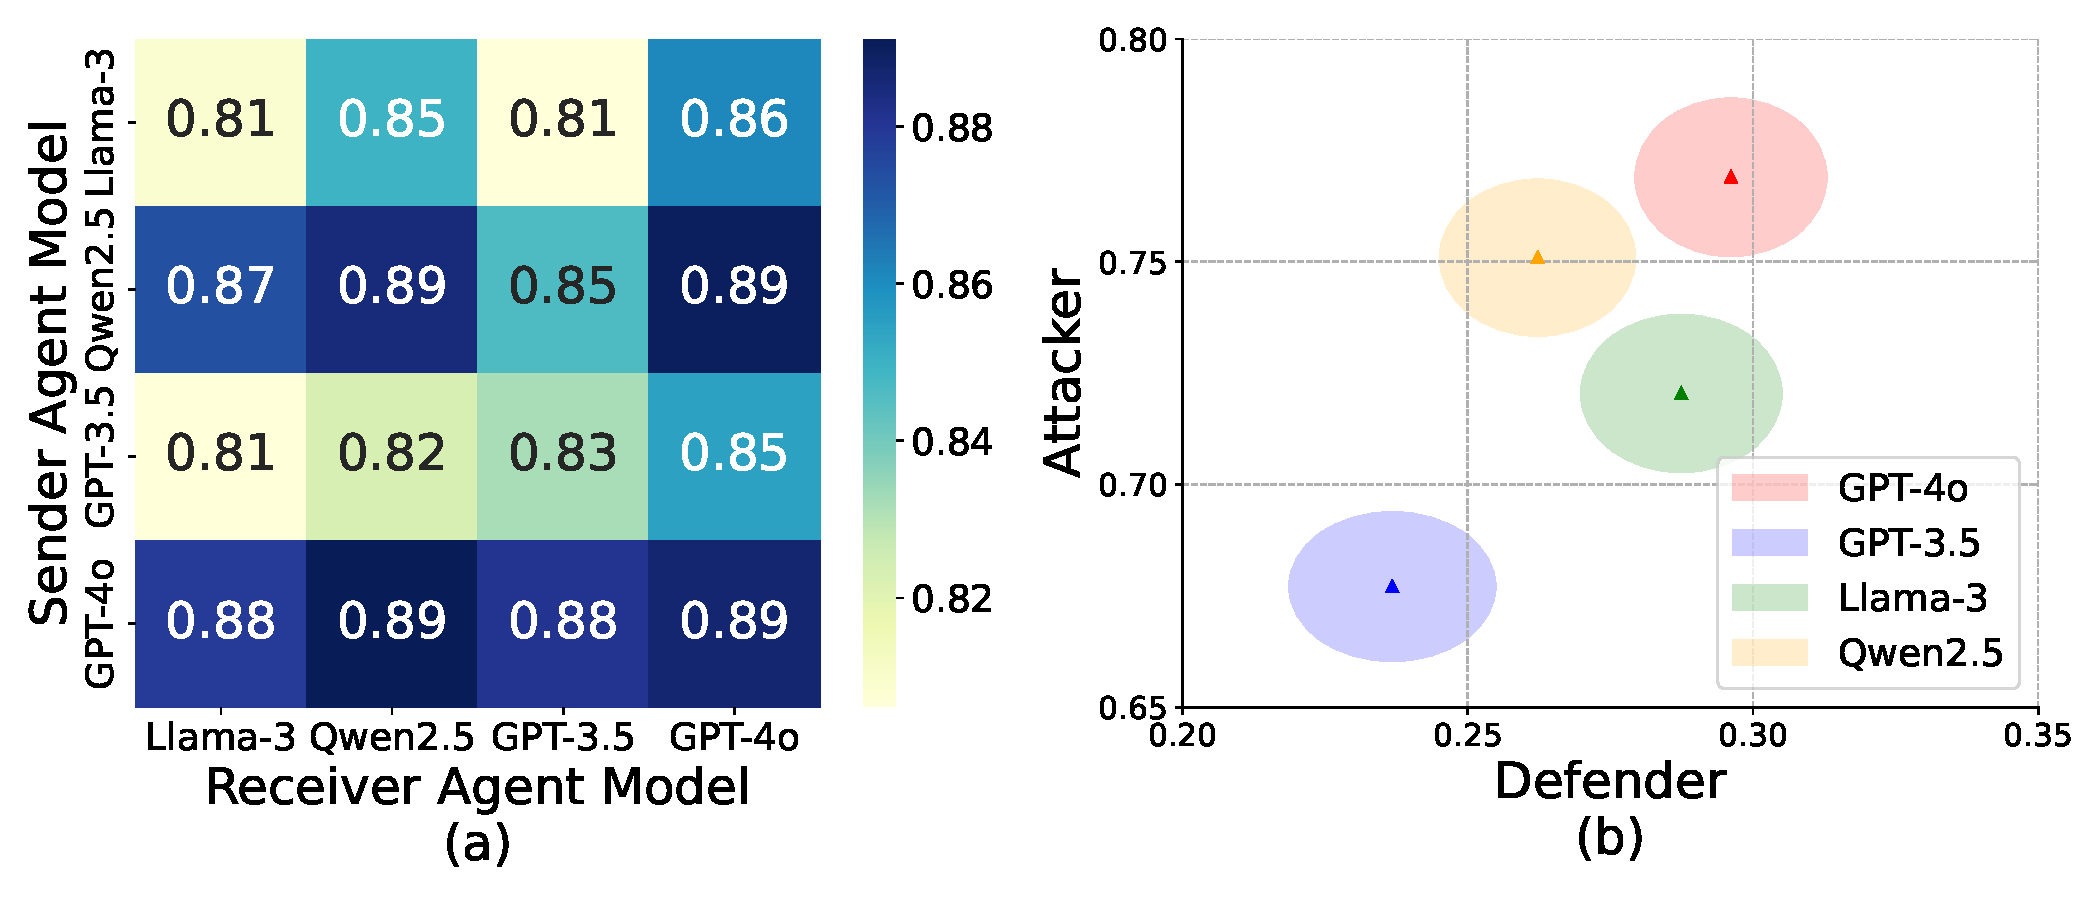
\includegraphics[width=\linewidth]{latex/figs/exp_ana.pdf}
    \caption{(a) Judge majority score of interactions among different model-driven agents, highlighting that being a sender is more challenging. (b) Model performance as both attacker and defender, with notably weaker and less consistent results when acting as a defender.}
    \label{fig:game_arena}
\end{figure}

\paragraph{Pairwise Model-based}
We also evaluate how agents perform when interacting with other agents supported by different models.
Given that our social scenarios can have more than two participants, we label each agent as either a \emph{sender} or a \emph{receiver} based on their social goals with the assistance of GPT-4o, inspired by the theory of communication~\cite{blau1964exchange,barnlund2017transactional}.
Senders share and transmit information, while receivers focus on understanding and responding.

Figure~\ref{fig:game_arena}(a) presents the overall results of such interactions.
GPT-4o and Qwen2.5-14b still perform best. However, \textbf{engaging with weaker models adversely affects all models' performance, particularly when the sender is the weaker agent.}
Our analysis (Appendix~\ref{app:heter_exp_res}) shows that weaker models struggle more as senders than as receivers This is because senders take a more active role in social interactions, making the associated tasks inherently more challenging.